\chapter{System Design}
\label{chapter_system_design}
\acresetall

This chapter portrays the design for the proposed implementation of the secure
ad hoc network.

\section{Requirements}
Ad hoc networks have some desired characteristics such as quick and inexpensive
setup and being independent of communication infrastructure, but they
also impose great challenges regarding security. The challenges
regarding security can vary depending the purpose and environment of the
network.

\subsection{Scenario}
The design and implementation presented in this thesis is mostly based on an
emergency situation scenario, in which communication infrastructure is
unavailable. This thesis will also reflect on some possible requirements given
by a military application.

If there is a major emergency situation such as an earthquake or tsunami, it is
likely that parts or the whole of the communication infrastructure at the scene
is destroyed or temporarily down. The remaining communication lines will then
probably be congested, such that little communication actually goes through.

In this situation, it is of great importance that Emergency Personnel, such as
Paramedics, Firemen, Policemen and the Military, are able to communicate
efficiently and therefore independently of the public communication
infrastructure. They need this network in order to manage the the operation, and
therefore availability is probably the most important trait of this network.
Secondly, they should be able to trust the communication on the network - i.e.
messages sent are from whom they claim they to be.

Also, being able to authorize new actors on the scene, such as Red Cross, can be
critical to the operation. These new actors will probably not have the necessary
authentication tokens, i.e. certificates, required by the authentication scheme
in the network.

\subsection{List of Requirements}
TODO: Use Martins requirement paper, add requirements, write about each one, not
only nr1 and 4.

Based on the scenario above these requirements can be extracted and made into
general requirements that needs to be addressed by the system design. The work
presented here is based on several sources, most prevalent being the research
from the OASIS project \cite{oasis_report} \cite{5683058} \cite{nyre2009secure}
and the doctoral project of Eli Winjum carried out at UniK
\cite{ffi_2005_04015}.

\begin{table}[ht!]
	\centering
	\begin{tabular}{ | l | p{11cm} | }
	\hline
	\textbf{Requirement} & \textbf{Requirement Description}\\\hline
		R1 & A node must be authorized in order to get full rights in a
		network \cite{dahill2001secure}, \cite{sanzgiri2002secure}\\\hline
		R2 & A node without a recognized authentication token should be able to become
		authorized if necessary\\ \hline
		R3 & Networks need a master node which handles access control\\\hline
		R4 & Different networks should be able to collaborate
		\cite{ffi_2005_04015}\\\hline
	\end{tabular}
	\caption{Requirements based upon our simplified and general scenario.}
	\label{tab:our_req}
\end{table}

An early study produced security requirements of ad hoc networks demanding
that the routing logic must not be spoofed or altered to produce different
behavior \cite{dahill2001secure}. This means authorization is required (R1)
before someone can partake in routing logic. FFI also requires seamless radio coverage over the
area giving us R4.

\section{Design Overview}
The secure ad hoc network designed here does not change any fundamental workings
of regular ad hoc routing protocols. Assuming all nodes in the network already
have been authenticated, the routing in the network should behave as if there
were no secure extension to the routing protocol.

The proposed design should work with most pro-active ad hoc routing protocols
with limited alterations - but this design is specifically made for the
BATMAN \cite{batman_rfc} routing protocol chosen for its simpler design compared to
e.g. OLSR \cite{clausen2003rfc3626} because it only uses the third layer of the
OSI Model \cite{zimmermann1980osi}. How to incorporate this design into BATMAN will be
expained in Chapter \ref{chapter_implementation}.

The basic principle of the proposed design is that an authenticated node accepts
other authenticated nodes' routing messages and forwards them as normal, while
discarding routing messages from unauthenticated nodes. One or more nodes in the
network will assume a role as master node(s), with the extra capability of
authorizing new nodes into the network. A special certificate called a \ac{PC}
\cite{tuecke2004rfc3820} will be used for authentication after this authorization has taken
place so other nodes in the network will be able to authenticate and accept the new
node.


\subsection{Entity Explanation}

Before a simplified example can be given, a few new entities in this design
needs to be explained further. This is the short version, just enough for the
reader to understand the example - the full description of these entities
and why they are necessary will be given later. All of these entities are also
portrayed in Figure \ref{fig:simple_example_entities}. The portrayed entities
will be used as a template for other figures later in this thesis report.

\begin{itemize}
  \item \textbf{\acf{SP}} is responsible for tasks similar to that of a \ac{CA}
  	and has the master role in the network. The \ac{SP} is the entity that
 	 authorizes new nodes and signs their \acp{PC}.
  \item \textbf{\acf{PC0}} is a self-signed \ac{PC} belonging to a
  	\ac{SP}. This \ac{PC} has a certificate depth of 0, thus we refer to it as a
  	\ac{PC0}.
  \item \textbf{\acf{PC1}} is a \ac{PC} signed by a \ac{PC0} (i.e. by the
  private key of the \ac{SP}). All authenticated nodes in one network, has a
  \ac{PC1} signed by a \ac{SP} from that network.
  \item \textbf{\acf{AL}} is a list containing the necessary information about
 	all authorized nodes in the network. The \ac{SP} signs and broadcasts a copy
 	of the \ac{AL} periodically, and all nodes keep a local copy of the \ac{AL}
  	which they use to authenticate other nodes in the network.
  \item \textbf{Authenticated Node} bla bla.
  \item \textbf{Unauthenticated Node} bla bla.
\end{itemize}

\begin{figure}[h]
	\centering
  	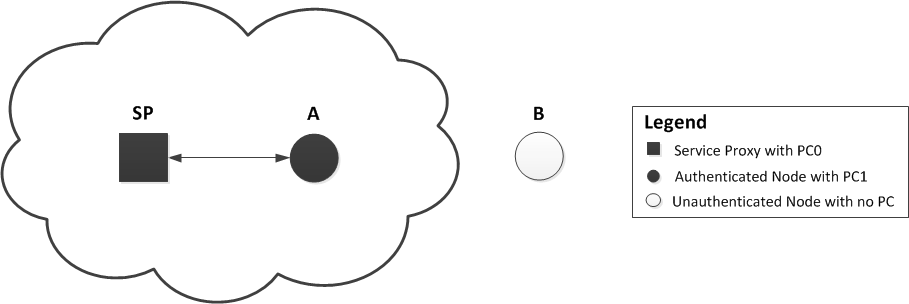
\includegraphics{images/simple_example_entities.png}
  	\caption{Different entities in the Simple Example.}
	\label{fig:simple_example_entities}
\end{figure}

\subsection{Simple Example}
TODO: Why proxy certs, and not just regular certs. Explain this very short in
this example.

Two nodes are within transmitting range of each other. One of the
nodes is a \ac{SP} and the other is unauthenticated. The pro-active ad hoc
routing protocol used on both nodes regularly broadcasts routing messages, so
the two nodes learn of each others' existence. Upon reception of a routing
message from the unauthenticated node, the \ac{SP} will invite the node for a
handshake. With this handshake, the unauthenticated node will send a \ac{PC}
request. The \ac{SP} can create and sign a \ac{PC} for this node - i.e. the node
is issued a \ac{PC1}.

Before the \ac{SP} actually signs the \ac{PC} requested from the unauthenticated
node, it needs some verification that the node is an actor that should be
allowed access to the network. The actor will therefore meet the \ac{SP} in the
field and give its public key fingerprint (out-of-band) so the \ac{SP} can
verify the incoming public key in the \ac{PC} request as the actor's request.

Using the public key of the \ac{PC1}, the newly trusted node will now create and 
broadcast a signature, and use an excerpt (offset value) from this signature
in its routing messages. The signature excerpt is just a value used in the
following routing messages, and not the cryptographic signature itself, but
will be used for recognition. This will be described further later in the
chapter. The \ac{SP}, recognizing the signature offset value will rebroadcast
the routing messages so regular ad hoc routing follows.

Also upon handshake completion is the generation an \ac{AL}. The \ac{SP} will
use this list in order to save certain necessary details about the other node,
such as its address, public key, last signature, and more. Also in this list is
the corresponding information about the \ac{SP} itself. When the list is created
or updated it is broadcasted to the network - signed by the \ac{SP} to ensure no
other node can alter the information about trusted nodes in the network.

Whenever a new node is discovered by the \ac{SP} this procedure repeats, and a
new addition is made to the \ac{AL}. Other previously trusted nodes will learn
the identity of new nodes when they receive the updated list from the \ac{SP}.

TODO: add an MSC or figure with the entities to explain the example\ldots

\section{Node States}
This section is devoted to explain the different states a node can be in, and
how it behaves during these different states. These states should be similar for
most pro-active routing protocols as the only thing triggering these phases are
the routing messages sent as per normal operation of any pro-active routing
protocol [some def of pro-active routing protocols].

\subsection{Node Discovery}
Upon entering the network area, the node is both unauthenticated and unknown to
the network. The node regularily broadcasts routing messages to be received by
any potential node in the area. Assume all nodes are configured with addresses
on the same subnet so they can receive the sent broadcast (See Limitations in
Section \ref{ip_address_conf}).

Simultaneously, the node also listens to other nodes' routing messages.
Depending on the time interval between the broadcasts and whether the nodes
within each other's transmitting range are asymmetrical, they will discover each
other approximately at the same time.

\begin{figure}[h]
	\centering
  	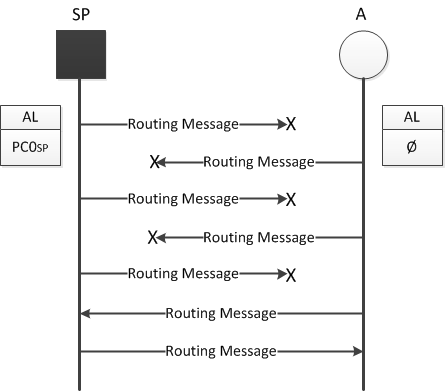
\includegraphics[width=0.5\textwidth]{images/node_states_discovery.png}
  	\caption{Discovery Phase between a \acf{SP} and an unauthenticated node (A)}
	\label{fig:node_states_discovery}
\end{figure}

Figure \ref{fig:node_states_discovery} illustrate the routing messages
periodically sent by two nodes until they discover each other. One of the nodes
have already assumed the master role and is a \ac{SP} while the other node is
unauthenticated.

The \ac{SP} will have its own self-issued (and signed) \ac{PC0} and its \ac{AL}
has only one entry - its own \ac{PC}. Note that if it had authorized another
node at an earlier point in time (but within the lifetime of the \ac{PC}) that
node's \ac{PC1} would also be represented in the \ac{AL}, even if the node was
outside the network at this point (physically).

The new node does not have any \ac{PC} at this point, unless it has a \ac{PC}
issued within and valid only for another network. This is however not covered
here, and it is assumed the node has no certificate at all. The same goes for
its \ac{AL}, or one can rather say it has an empty \ac{AL} - denoted by the '�'
in the figure.

\subsection{Authentication Handshake}
Once the two nodes have discovered each other, they will enter the
authentication handshake state. Note that while the nodes are executing the
authentication handshake, they will also continue to execute the regular routing
operations because this authentication step will be executed in a separate
thread. This is further elaborated in the next chapter.

The unknown node will wait for a predefined amount of time, for it is not
necessary that it will ever receive a request. The discovery might have been of
an authenticated node with a \ac{PC1} and not a \ac{SP}, which does not have the
rights to authenticate new nodes. It might also have been that of a \ac{SP}, but
because of the flaky nature of ad hoc networks, the two nodes might have become
invisible to each other before the handshake could be initiated.

While the new node is waiting for an invite, the \ac{SP} generate the invite
message which is a message containing the public key, i.e. the \ac{PC0}, and a
list of requirements regarding the allowed cryptographic encryption schemes, key
sizes and so on. The \ac{SP} will then send the invite directly addressed to the
new node. The \ac{SP} will then wait for a certificate request (\ac{PC} Request)
for a predefined time before re-sending the invite. It will do this at a maximum
three(TODO: maybe find a source claiming a number of times is better based on
statistics or whatever..) times before aborting the authentication handshake
with the new node.

Based on the requirements set by the \ac{SP} in the invite message, the new node
will generate an asymmetric key pair and a \ac{PC} request which it will send
back. This request abides by the rules for making a proxy certificate
\cite{rfc3820}, setting the Issuer Name as the Subject Name from the received
\ac{PC0}, the Subject Name as the Issuer Name appended with its own unique
Common Name from a hash of its own public key, and the Serial Number from the
same hash value. Why proxy certificates are used will be discussed later.

As Figure \ref{fig:node_states_handshake} shows, the last message to be sent in
the handshake is the actual signed certificate (\ac{PC1}) from the \ac{SP} to
the new node. At this point the \ac{SP} will add the \ac{PC1} to its local
\ac{AL} (which will be broadcasted later) and the new node will store the
certificate for making signatures later.

\begin{figure}[h]
	\centering
  	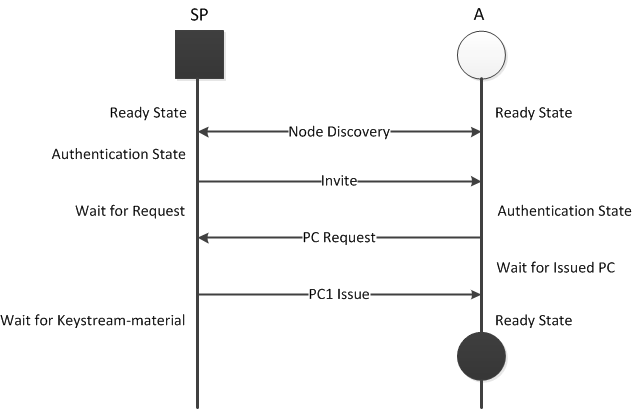
\includegraphics[width=0.5\textwidth]{images/node_states_handshake.png}
  	\caption{Handshake between a \acf{SP} and an unauthenticated node (A).}
	\label{fig:node_states_handshake}
\end{figure}

\subsubsection*{Out-Of-Band}
In the section above the different states and messages shared between the two
nodes were discussed. How and and on what grounds the \ac{SP} accepts the
\ac{PC} request from the new node however, was not discussed. There are many
possible authentication schemes, but when it comes to \acp{MANET}, possibly with
no Internet connection, proper authentication becomes a difficult task. In
the discussion in Chapter \ref{chapter_discussion} different schemes will be
discussed, but here only one scheme is accounted for.

If you have no pre-shared information between the parties involved in the
network, the simplest way to authenticate a new node is to use an out-of-band
authentication. The implementation of such an authentication scheme will be
discussed in the next chapter, and will only be briefly mentioned here.

New users will have to use share their public key fingerprint with the \ac{SP}
physically, and vice versa. By doing this, the \ac{SP} can store the fingerprint
and use it to check the received public key in the \ac{PC} request for
authenticity in order to make sure the new node is run by the actual person he
met and verified physically. The new node can similarily verify the \ac{SP}.

\subsection{Authorized Operation}
Once a node is authorized and has its own \ac{PC1}, it can send its own routing
announcements, receive announcements, and forward other nodes' announcements.
This means that the node is a fully worthy member of the MANET. However, there
is one thing missing before the node can be verified and verify other nodes
(than the \ac{SP}) - i.e. it has to learn the public key and address of all its
neighbors.

Figure \ref{fig:node_states_authorized} shows the authorized node receiving
an \ac{AL} Update from the \ac{SP}. This message contains the full \ac{AL} list
and lets the newly authorized node learn the public key and address of potential
other nodes in the network. The list is broadcasted by the \ac{SP} periodically
to make sure all nodes in the network know and trust each other.

\begin{figure}[h]
	\centering
  	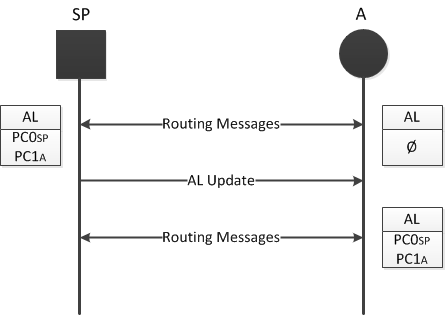
\includegraphics[width=0.5\textwidth]{images/node_states_authorized.png}
  	\caption{Normal operation between a \acf{SP} and an unauthenticated node
  	(A)including an \ac{AL} Update message.}
	\label{fig:node_states_authorized}
\end{figure}



\subsubsection*{Discovering New Nodes}